\section{Camera calibration and pose estimation}
Camera calibration is carried out using open-source computer vision library OpenCV \cite{OpenCV}. Camera calibration is based on 2D/2D point correspondences with the chessboard as a 2D planar object. The homography is calculated using square corners of a chessboard (world points) and its image points. OpenCV needs an arrays of world points and image points and the grid size of the chessboard (in our case its 5 rows, 8 columns). Therefore, 10 RGB images of the chessboard at different position and orientation was recorded and an array of world points (x,y) location of chessboard corners [(0,0), (40,0), (80,0)...] was fed to the algorithm. OpenCV automatically detects these chessboard corners from the images as shown in \cref{fig:chessboard_corners} and refines them accordingly.

\begin{figure}[hbt!]
	\centering
	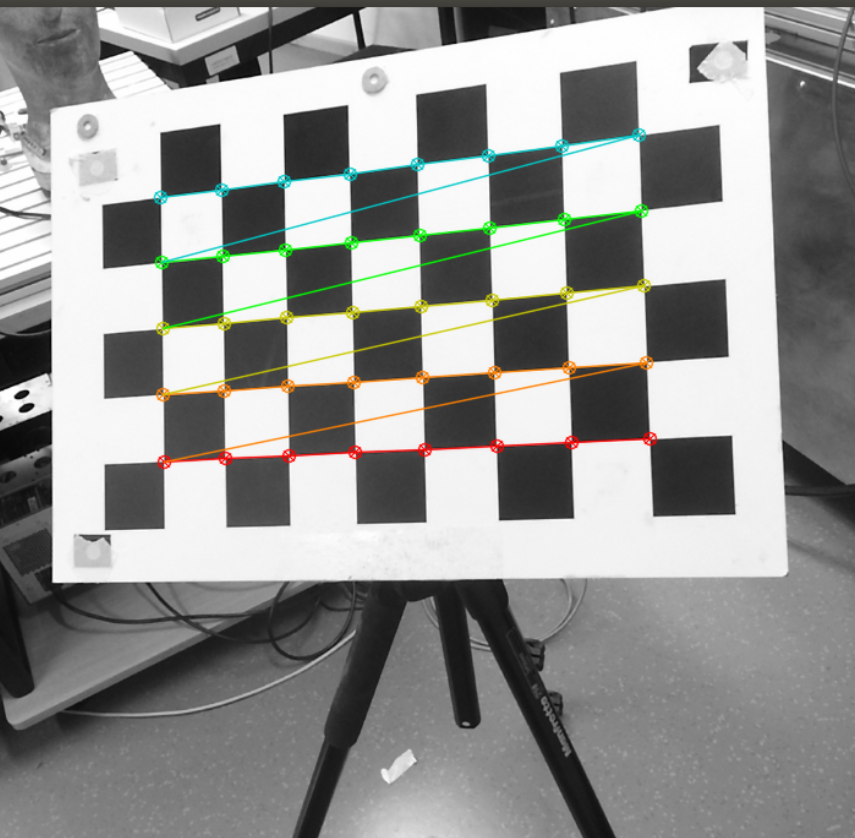
\includegraphics[scale=0.6]{chessboard_corners.png}
	\caption{Chessboard corners(image points) detection in OpenCV}
	\label{fig:chessboard_corners}
\end{figure}

\begingroup\makeatletter\def\@currenvir{verbatim}
\verbatim
cv2.calibrateCamera(object_points, image_points, ...)
output: rms, camera_matrix, dist_coeffs, rot_vecs, trans_vecs
\end{verbatim}

The OpenCV function cv2.calibrateCamera takes in these world points (object points), image points and some more arguements then outputs geometric error of reprojection (rms), intrinsic parameters (camera\_matrix) distortion coefficients (dist\_coeffs) and extrinsic parameters $(rot\_vecs, trans\_vecs)$.

Having completed the camera calibration we can now make use of the intrinsic parameters and the distortion coefficients as an input to the pose estimation algorithm provided by OpenCV. 

\begingroup\makeatletter\def\@currenvir{verbatim}
\verbatim
cv2.solvePnP(object_points, image_points, intr_mat, dist_coeffs)
output: rot_vecs, trans_vecs 
\end{verbatim}


The OpenCV function cv2.solvePnP takes object points, image points, intrinsic matrix, and distortion coeffcients as the arguments and computes rotation and translation vectors. Rotation vector can be converted to 3$\times$3 rotational matrix using cv2.Rodrigues function provided by openCV. By combining rotation matrix and translation vector we can form 4$\times$4 homogenious matrix for further manipulation.